\subsection{Vorbereitungsaufgabe}
Zunächst werden die Fourierkoeffizienten der Rechteck-, Dreieck- und Sägezahnspannung berechnet.

\subsection{Fourieranalyse}
Die Schaltung wird wie folgt aufgebaut:
\begin{figure}[h!]
  \centering
  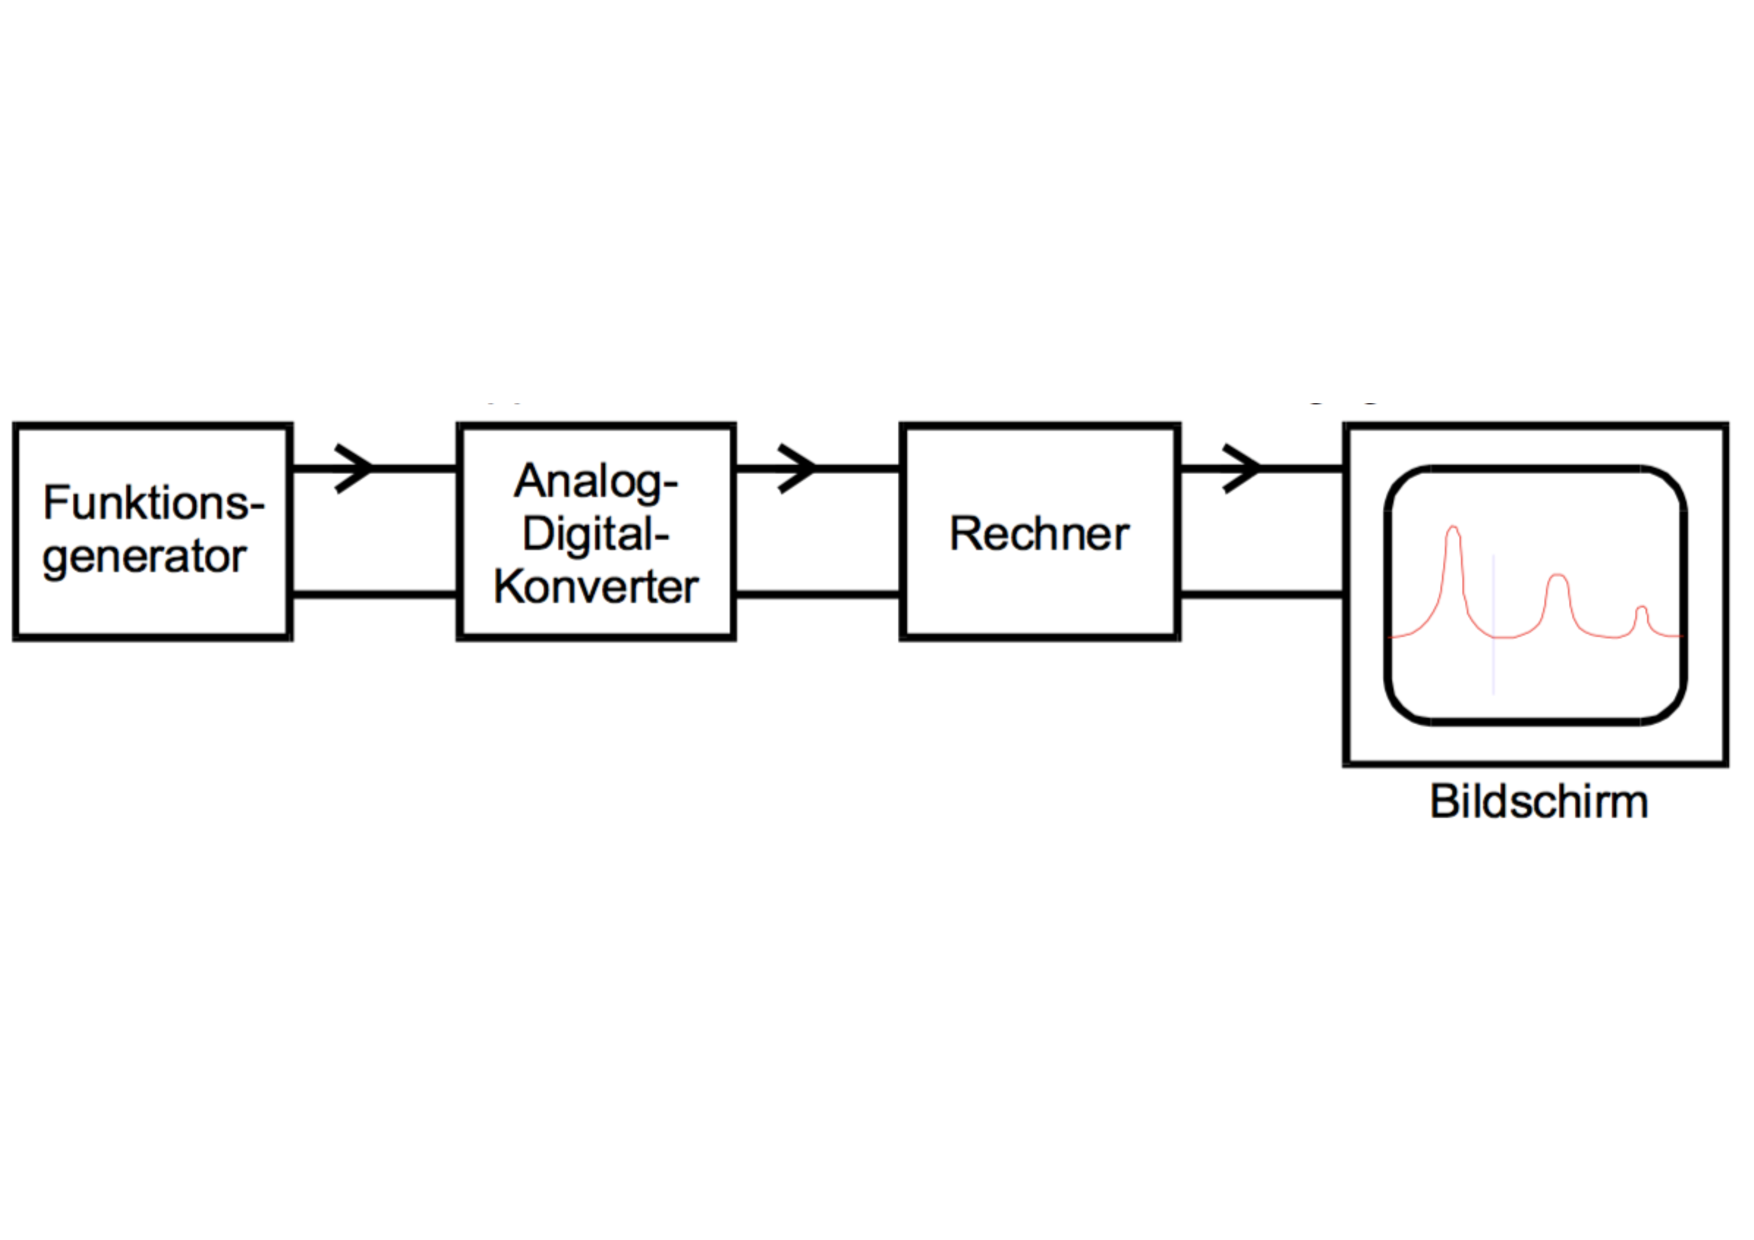
\includegraphics[width=\textwidth]{transformation.pdf}
  \caption{Schema des Versuchaufbaus zur Fourieranalyse \cite{1}}
  \label{fig:transformation}
\end{figure}
Der Analog-Digital-Konverter, der Rechner und der Bildschirm sind im Oszilloskop integriert.
Als erstes wird mit dem Spannungsgenerator eine periodische Spannung eingespeist.
Am Oszilloskop wird die Spannung sichtbar gemacht.
Mit der Math-Funktion des Ozsilloskops wird das Linienspektrum dargestellt.
Mithilfe des Cursors werden möglichst viele Amplituden des Linienspektrums abgemessen.
Die Messung wird für eine Rechteckspannung, eine Dreieckspannung und eine Sägezahnspannung durchgeführt.
Bei der Rechteckspannung werden neun Werte gemessen, bei der Dreieckspannung wird die Messung ab dem achtem Peak sehr ungenau.
Für die Sägezahnspannung werden neun Werte abgelesen.

\subsection{Fouriersynthese}
Für die Fouriersynthese werden ein Oberwellengenerator und ein Voltmeter zur Schaltung hinzugefügt.
\\Mithilfe der Lissajousfiguren wird die Amplitude und Phasenverschiebung der einzelnen Oberwellen angepasst.
Dazu wird das Oszilloskop auf den X-Y-Modus ungeschaltet.
\\Es wird stets die erste Oberwelle mit einer höheren Oberwelle auf dem Oszilloskop dargestellt.
Mit der richtigen Phasenverschiebung bilden sich die Lissajousfiguren aus.
Damit sind die Ausgänge alle in der richtigen Phase für die Fouriersynthese.
\\Mit dem Voltmeter und dem Spannungsgenerator werden nun die in der Vorbereitungsaufgabe berechneten Spannungen möglichst genau eingeregelt.
Für die Synthetisierung der Rechteckspannung und der Dreieckspannung werden nur die ungeraden Oberwellen benötigt.
Somit werden für die Rechteckspannung und für die Dreieckspannung fünf Werte aufgenommen, für die Sägezahnspannung zehn Werte.
